\documentclass[a4paper]{tufte-handout}

% --- BUG FIX FOR TUFTE-LATEX ---
% Tufte hasn't been updated to support modern LaTeX case-changing engines.
% This dummy command stops Tufte from crashing when it builds the page headers.
\renewcommand{\MakeTextLowercase}[1]{#1}
% -------------------------------

\title[Sound]{Sound\thanks{Draft version as of \today}}
\author[dishajk]{Disha Kuzhively}

\usepackage{tikz}

% Standardize command font styles and environments
\newcommand{\doccmd}[1]{\texttt{\textbackslash#1}}
\newcommand{\docopt}[1]{\ensuremath{\langle}\textrm{\textit{#1}}\ensuremath{\rangle}}
\newcommand{\docarg}[1]{\textrm{\textit{#1}}}
\newcommand{\docenv}[1]{\textsf{#1}}
\newcommand{\docpkg}[1]{\texttt{#1}}
\newcommand{\doccls}[1]{\texttt{#1}}
\newcommand{\docclsopt}[1]{\texttt{#1}}
\newenvironment{docspec}{\begin{quote}\noindent}{\end{quote}}
\usepackage{textcase}
\let\MakeTextLowercase\relax
\let\MakeTextUppercase\relax
\begin{document}

\maketitle

\begin{abstract}
\noindent
This article was prepared by the author to serve as a draft for TNSCERT class 8 chapter on the concept of Sound for TNSCERT during the the Tamil Nadu Curriculum Framing(TNCF) workshop that was held in Asha Nivas, Chennai  from 13-11-2025 to 15-11-2025, and 09-03-2026 to 10-03-2026.

The right side margin of each page contains notes for teachers, and prompts to activities that the teacher can initiate in the classroom.
\end{abstract}

Every day we experience many natural and human-made sounds around us. At night, we may hear the soft chirping of crickets. At dawn, the sweet chirping of birds welcomes a new day. As the town wakes up, we hear the sounds of buses, cars, two-wheelers, and the honking of horns. In school, the ringing of the bell tells us when a class begins or ends. We also hear raindrops falling on the ground, a dog barking, or a phone ringing.

Where do these sounds come from? In this chapter, we will explore how sound is produced and how it propagates\footnote{Here the word 'propagate' is used instead of simpler and familiar word like 'travel' to avoid misconceptions that students create, e.g. The word travel suggests that 'sound' is a moving object. Words are chosen to ensure that students develop a scientifically accurate mental model of the concept.} from one place to another. We will also learn that sound can be understood as a wave.
\newthought{Exercise: }Close your eyes for one minute and listen carefully. Write down all the sounds you hear.

\subsection{Activity: Vibrating Scale}
Materials required:
\begin{enumerate}
    \item Scale
    \item Desk or table
\end{enumerate}
\newthought{Procedure:} Place the scale on the desk so that about one-third of it is over the edge. Hold the part of the scale resting on the desk with one hand. Push the free end of the scale downward. Release the scale quickly.
\begin{marginfigure}
  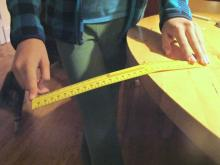
\includegraphics{scale-down}
  \caption[Sound with a scale]{Step 1. Push the free end of the scale downwards.}
\end{marginfigure}
\marginnote{\footnotesize Image credit: Ingrid Sulston, licensed under CC BY-NC-SA 4.0}
\begin{marginfigure}
  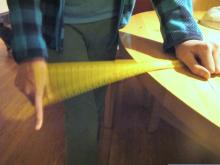
\includegraphics{scale-vibrate}
  \caption[Sound with a scale]{Step 2. Let the pushed end go.}
\end{marginfigure}
\marginnote{\footnotesize Image credit: Ingrid Sulston, licensed under CC BY-NC-SA 4.0}
\newthought{Observe:} What happens to the free end of the scale? Do you hear a sound? Do you see the scale move up and down rapidly? What type of motion is this?

\subsection{Activity: Rubber Band Instrument}
Materials required:
\begin{enumerate}
    \item Rubber bands
    \item Geometry box
    \item Two pens or pencils
\end{enumerate}
\begin{marginfigure}
  \centering
\begin{tikzpicture}
    \node[draw] at (0,0) {Image of a pencil box with a rubber band around it.};
  \end{tikzpicture}
  \caption{Pencil box with rubber band around it.}
  \label{rubberbox}
\end{marginfigure}
\newthought{Procedure:} Close the geometry box. Stretch a rubber band across the length of the box. Place a pencil each under the rubber band near the two ends. This will lift the rubber band slightly above the surface of the box. See Figure~\ref{rubberbox}. Pluck the rubber band with your finger.

\end{document}